\documentclass[a4paper,11pt]{report}
\usepackage{chuan_math_gkt}
\usetikzlibrary{angles,quotes,intersections,patterns,decorations.pathreplacing}
\chuanexamsetup

\begin{document}
\examfontsize

\examsecret{绝密$\bigstar$启用前}

\examtitle{2021年普通高等学校招生全国统一考试（天津卷）}{数\quad 学}

\noticetitle
\begin{examnotice}
\item 答卷前，考生务必将自己的姓名、准考证号填写在答题卡上。
\item 回答选择题时，选出每小题的答案后，用铅笔把答题卡上对应题目的答案标号涂黑。如需改动，用橡皮擦干净后，再选涂其他答案标号。回答非选择题时，将答案写在答题卡上。写在本试卷上无效。
\item 考试结束后，将本试卷和答题卡一并交回。
\end{examnotice}

\examsection{一、选择题：本大题共9小题，每小题5分，共45分。在每小题给出的四个选项中，只有一项是符合题目要求的。}
\begin{examquestions}

\item 设集合 $A=\{-1,0,1\}$，$B=\{1,3,5\}$，$C=\{0,2,4\}$，则 $(A\cap B)\cup C=$
\fourchoices{$\{0\}$}{$\{0,1,3,5\}$}{$\{0,1,2,4\}$}{$\{0,2,3,4\}$}
\item 已知 $a\in\mathbb R$，则“$a>6$”是“$a^2>36$”的
\twochoices{充分不必要条件}{必要不充分条件}{充要条件}{既不充分也不必要条件}
\item 函数 $y=\dfrac{\ln|x|}{x^2+2}$ 的图像大致为
\graphchoices{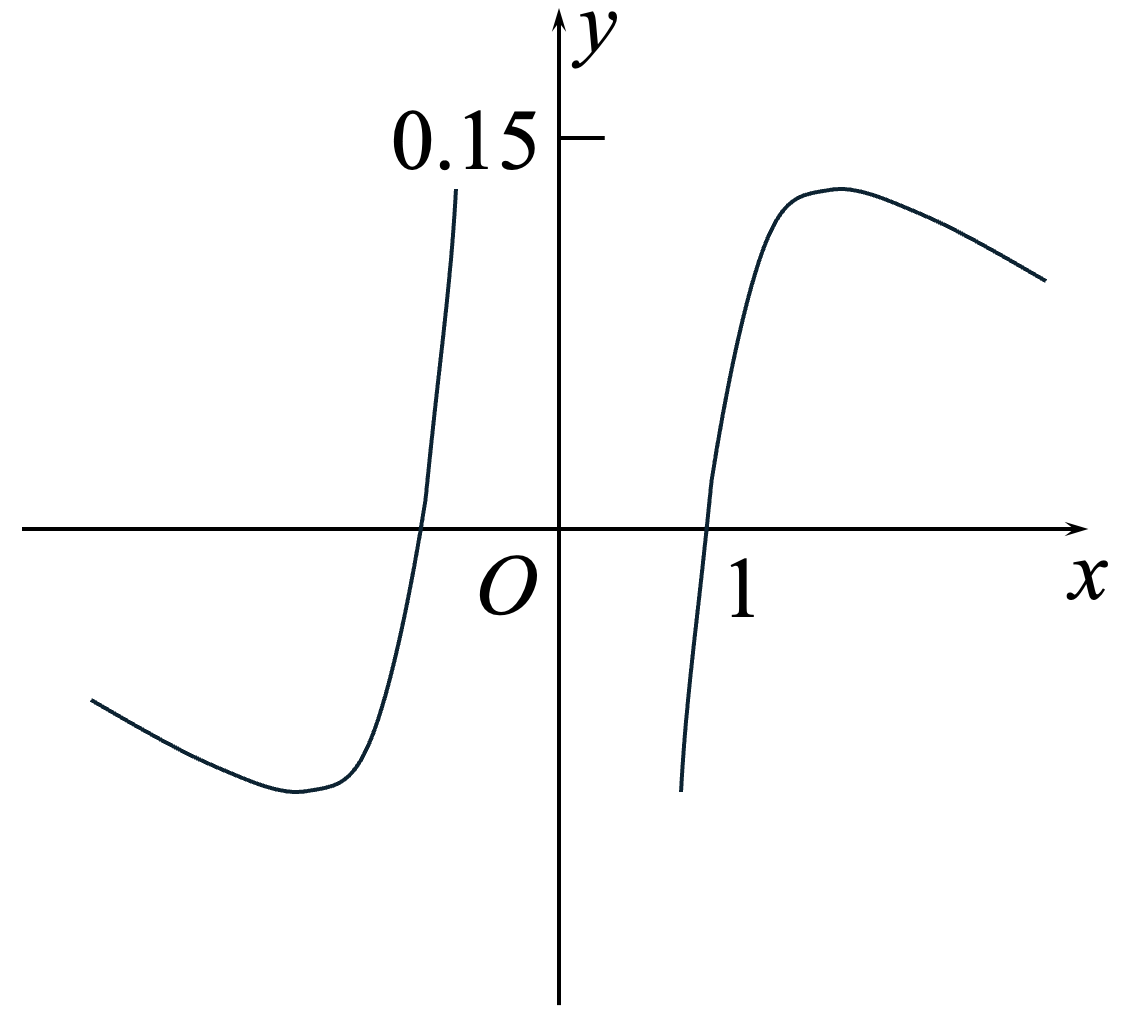
\includegraphics[width=4.0cm]{figures/2021_tj_q3_A.png}}{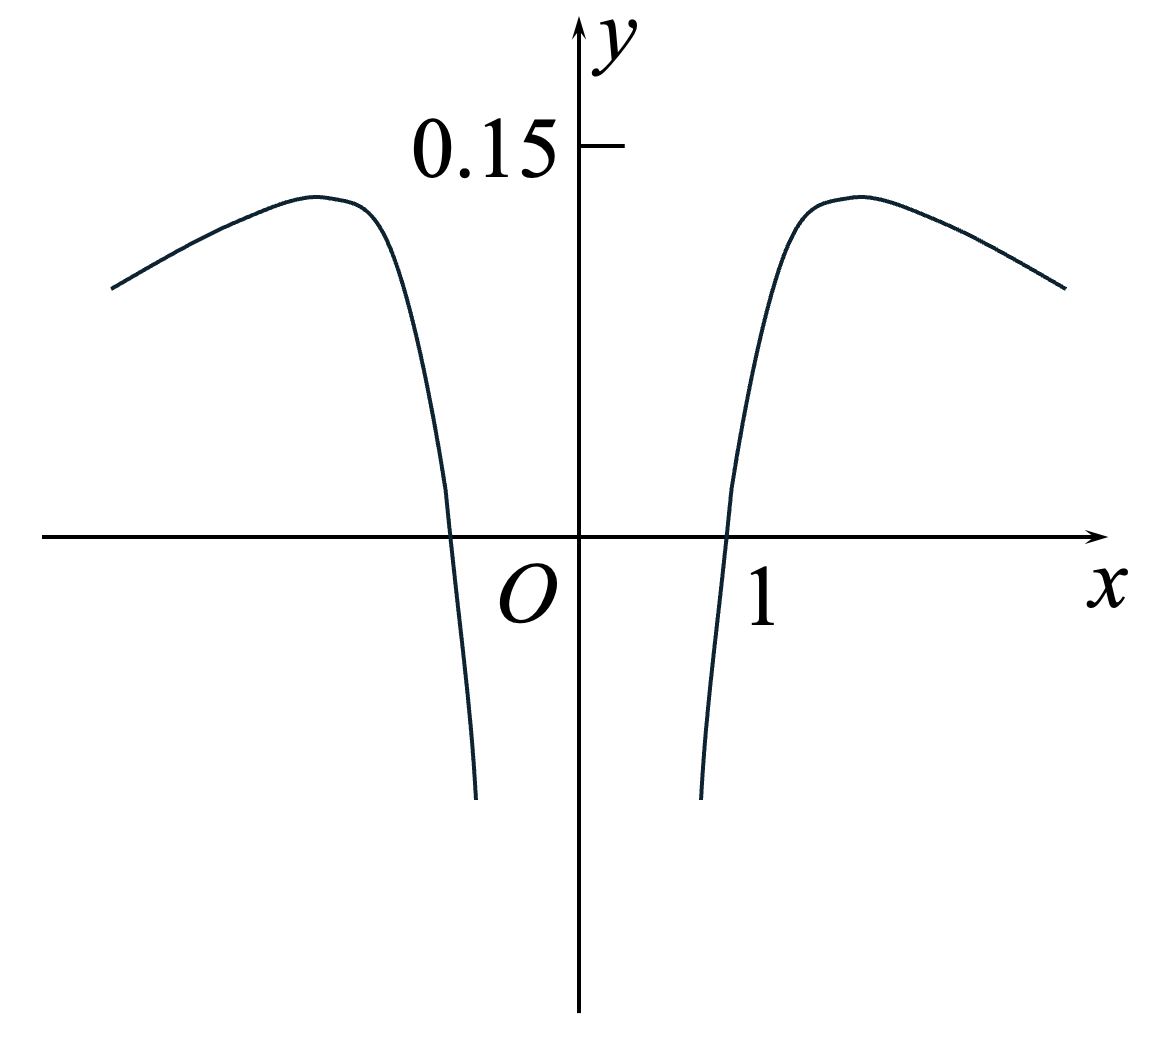
\includegraphics[width=4.0cm]{figures/2021_tj_q3_B.png}}{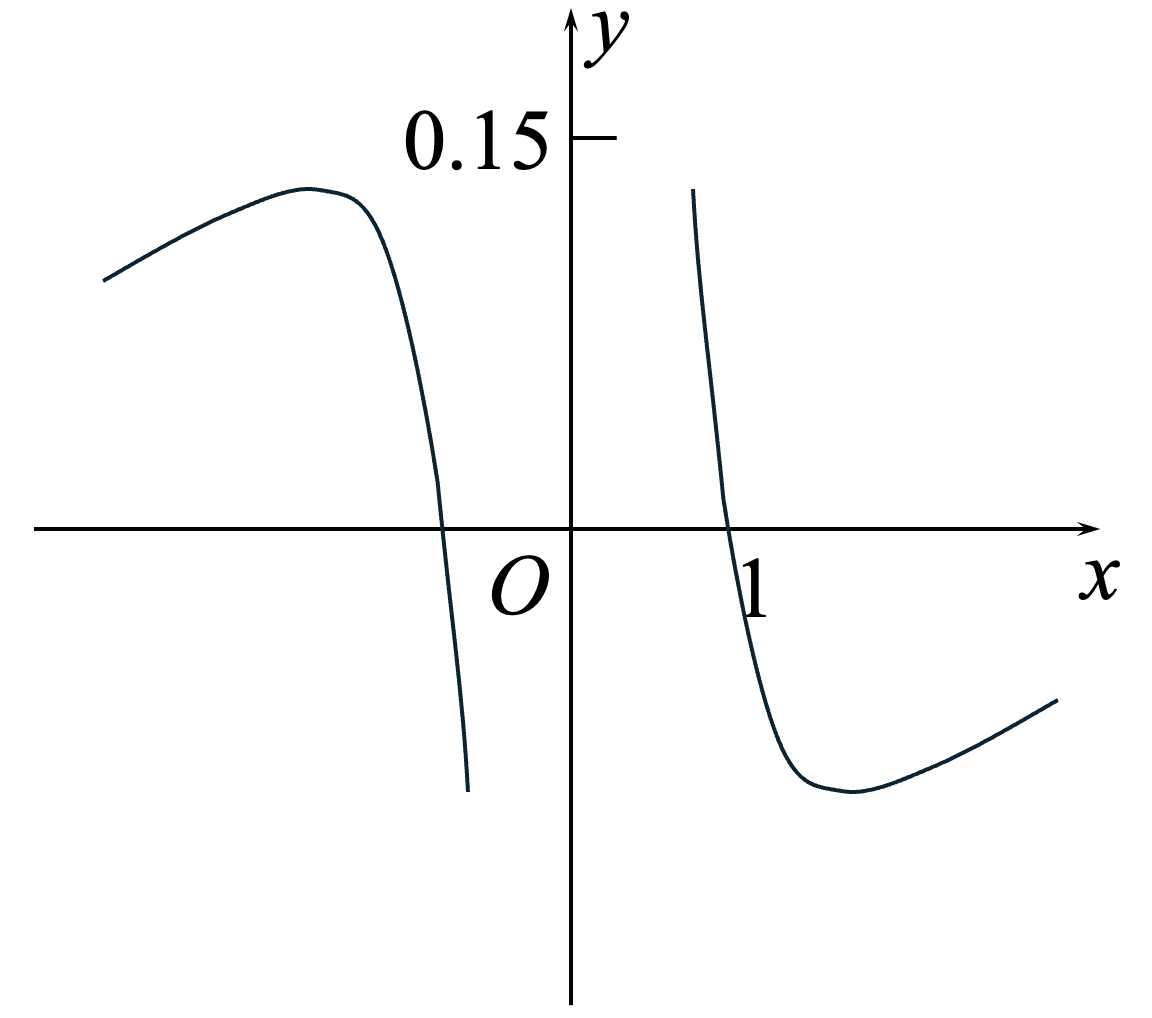
\includegraphics[width=4.0cm]{figures/2021_tj_q3_C.png}}{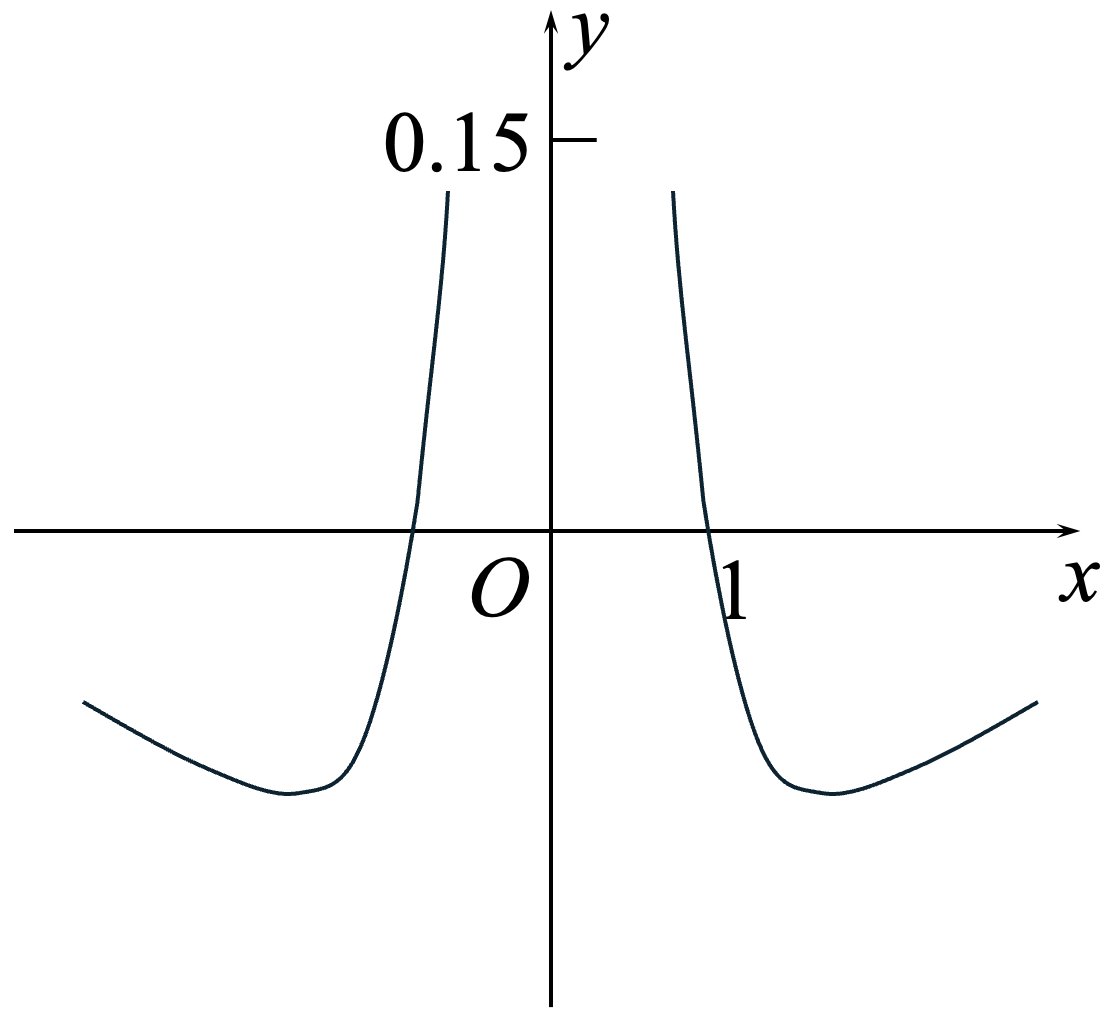
\includegraphics[width=4.0cm]{figures/2021_tj_q3_D.png}}
\item 从某网格平台推荐的影视作品中抽取 $400$ 部，统计其评分分数据，将所得 $400$ 个评分数据分为 $8$ 组：$[66,70),[70,74),\ldots,[94,98]$，并整理得到如下的频率分布直方图，则评分在区间 $[82,86)$ 内的影视作品数量是
\begin{tightcenter}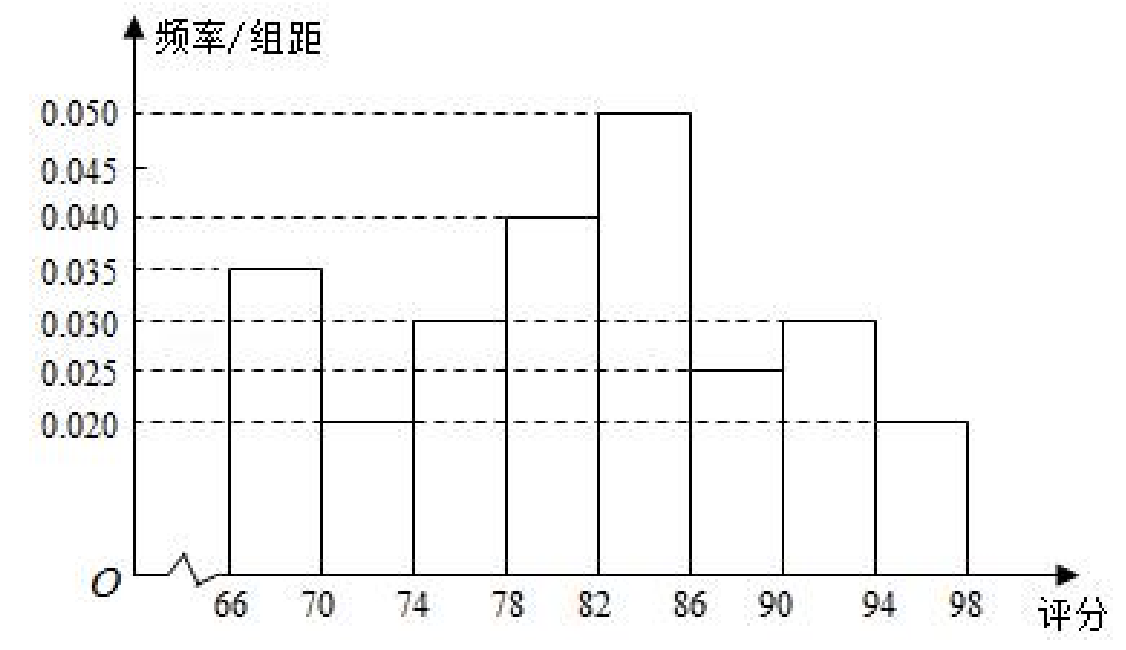
\includegraphics[width=8.0cm]{figures/2021_tj_q4.png}\end{tightcenter}
\fourchoices{$20$}{$40$}{$64$}{$80$}
\item 设 $a=\log_2 0.3$，$b=\log_{\frac12}0.4$，$c=0.4^{0.3}$，则 $a,b,c$ 的大小关系为
\fourchoices{$a<b<c$}{$c<a<b$}{$b<c<a$}{$a<c<b$}
\item 两个圆锥的底面是一个球的同一截面，顶点均在球面上，若球的体积为 $\dfrac{32\pi}{3}$，两个圆锥的高之比为 $1:3$，则这两个圆锥的体积之和为
\fourchoices{$3\pi$}{$4\pi$}{$9\pi$}{$12\pi$}
\item 若 $2^a=5^b=10$，则 $\dfrac1a+\dfrac1b=$
\fourchoices{$-1$}{$\lg7$}{$1$}{$\log_710$}
\item 已知双曲线 $\dfrac{x^2}{a^2}-\dfrac{y^2}{b^2}=1(a>0,b>0)$ 的右焦点与抛物线 $y^2=2px(p>0)$ 的焦点重合，抛物线的准线交双曲线于 $A,B$ 两点，交双曲线的渐近线于 $C,D$ 两点，若 $|CD|=\sqrt2|AB|$，则双曲线的离心率为
\fourchoices{$\sqrt2$}{$\sqrt3$}{$2$}{$3$}
\item 设 $a\in\mathbb R$，函数 $f(x)=\linsys{\cos(2\pi x-2\pi a),\quad x<a,\\x^2-2(a+1)x+a^2+5,\quad x\geq a}$，若 $f(x)$ 在区间 $(0,+\infty)$ 内恰有 $6$ 个零点，则 $a$ 的取值范围是
\twochoices{$\left(2,\dfrac94\right]\cup\left[\dfrac52,\dfrac{11}4\right)$}{$\left(\dfrac74,2\right)\cup\left(\dfrac52,\dfrac{11}4\right)$}{$\left(2,\dfrac94\right]\cup\left[\dfrac{11}4,3\right)$}{$\left(\dfrac74,2\right)\cup\left[\dfrac{11}4,3\right)$}

\end{examquestions}

\examsection{二、填空题：本大题共6小题，每小题5分，共30分。试题中包含两个空的，答对1个的给3分，全部答对的给5分。}
\begin{examquestions}[start=10]

\item $\mathrm{i}$ 是虚数单位，复数 $\dfrac{9+2\mathrm{i}}{2+\mathrm{i}}=$\blank。
\item 在 $\left(2x^3+\dfrac1x\right)^6$ 的展开式中，$x^6$ 的系数是\blank。
\item 若斜率为 $\sqrt3$ 的直线与 $y$ 轴交于点 $A$，与圆 $x^2+(y-1)^2=1$ 相切于点 $B$，则 $|AB|=$\blank。
\item 若 $a>0$，$b>0$，则 $\dfrac1a+\dfrac a{b^2}+b$ 的最小值为\blank。
\item 甲、乙两人在每次猜谜活动中各猜一个谜语，若一方猜对且另一方猜错，则猜对的一方获胜，否则本次平局。已知每次活动中，甲、乙猜对的概率分别为 $\dfrac56$ 和 $\dfrac15$，且每次活动中甲、乙猜对与否互不影响，各次活动也互不影响，则一次活动中，甲获胜的概率为\blank，$3$ 次活动中，甲至少获胜 $2$ 次的概率为\blank。
\item 在边长为 $1$ 的等边三角形 $ABC$ 中，$D$ 为线段 $BC$ 上的动点，$DE\perp AB$ 且交 $AB$ 于点 $E$，$DF\parallel AB$ 且交 $AC$ 于点 $F$，则 $|2\overrightarrow{BE}+\overrightarrow{DF}|$ 的值为\blank；$(\overrightarrow{DE}+\overrightarrow{DF})\cdot\overrightarrow{DA}$ 的最小值为\blank。

\end{examquestions}

\examsection{三、解答题：本大题共5小题，共75分。解答应写出文字说明、证明过程或演算步骤。}
\begin{examanswers}[start=16]

\item（14分）

在 $\triangle ABC$ 中，角 $A,B,C$ 所对的边分别为 $a,b,c$，已知 $\sin A:\sin B:\sin C=2:1:\sqrt2$，$b=\sqrt2$。

（1）求 $a$ 的值；（2）求 $\cos C$ 的值；（3）求 $\sin\left(2C-\dfrac\pi6\right)$ 的值。

\item（15分）

如图，在棱长为 $2$ 的正方体 $ABCD-A_1B_1C_1D_1$ 中，$E$ 为棱 $BC$ 的中点，$F$ 为棱 $CD$ 的中点。

\noindent\begin{minipage}[t]{0.64\linewidth}
（1）求证：$D_1F\parallel$ 平面 $A_1EC_1$；

（2）求直线 $AC_1$ 与平面 $A_1EC_1$ 所成角的正弦值；

（3）求二面角 $A-AC_1-E$ 的正弦值。
\end{minipage}\hfill
\begin{minipage}[t]{0.30\linewidth}\vspace{-1.0em}\centering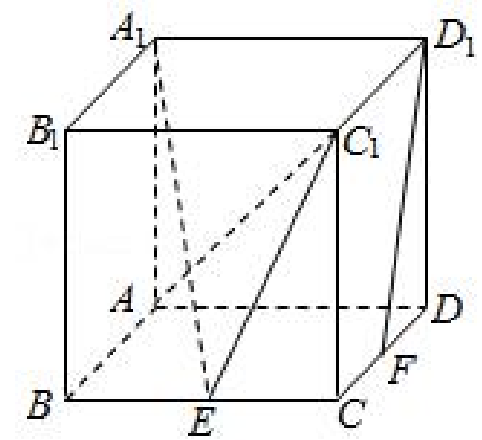
\includegraphics[width=\linewidth]{figures/2021_tj_q17.png}\end{minipage}
\newpage
\item（15分）

已知椭圆 $\dfrac{x^2}{a^2}+\dfrac{y^2}{b^2}=1(a>b>0)$ 的右焦点为 $F$，上顶点为 $B$，离心率为 $\dfrac{2\sqrt5}{5}$，且 $|BF|=\sqrt5$。

（1）求椭圆的方程；

（2）直线 $l$ 与椭圆有唯一的公共点 $M$，与 $y$ 轴的正半轴交于点 $N$，过 $N$ 与 $BF$ 垂直的直线交 $x$ 轴于点 $P$。若 $MP\parallel BF$，求直线 $l$ 的方程。

\item（15分）

已知 $\{a_n\}$ 是公差为 $2$ 的等差数列，其前 $8$ 项和为 $64$，$\{b_n\}$ 是公比大于 $0$ 的等比数列，$b_1=4$，$b_3-b_2=48$。

（1）求 $\{a_n\}$ 和 $\{b_n\}$ 的通项公式；

（2）记 $c_n=b_{2n}+\dfrac1{b_n}$，$n\in\mathbb N^*$。

（i）证明 $\{c_n^2-c_{2n}\}$ 是等比数列；

（ii）证明 $\displaystyle\sum_{k=1}^n\sqrt{\dfrac{a_ka_{k+1}}{c_k^2-c_{2k}}}<2\sqrt2$。

\item（16分）

已知 $a>0$，函数 $f(x)=ax-xe^x$。

（1）求曲线 $y=f(x)$ 在点 $(0,f(0))$ 处的切线方程；

（2）证明 $f(x)$ 存在唯一的极值点；

（3）若存在 $a$，使得 $f(x)\leq a+b$ 对任意 $x\in\mathbb R$ 成立，求实数 $b$ 的取值范围。

\end{examanswers}

\end{document}
